\documentclass[]{article}
\usepackage{lmodern}
\usepackage{amssymb,amsmath}
\usepackage{ifxetex,ifluatex}
\usepackage{fixltx2e} % provides \textsubscript
\ifnum 0\ifxetex 1\fi\ifluatex 1\fi=0 % if pdftex
  \usepackage[T1]{fontenc}
  \usepackage[utf8]{inputenc}
\else % if luatex or xelatex
  \ifxetex
    \usepackage{mathspec}
    \usepackage{xltxtra,xunicode}
  \else
    \usepackage{fontspec}
  \fi
  \defaultfontfeatures{Mapping=tex-text,Scale=MatchLowercase}
  \newcommand{\euro}{€}
\fi
% use upquote if available, for straight quotes in verbatim environments
\IfFileExists{upquote.sty}{\usepackage{upquote}}{}
% use microtype if available
\IfFileExists{microtype.sty}{\usepackage{microtype}}{}
\usepackage{graphicx}
\makeatletter
\def\maxwidth{\ifdim\Gin@nat@width>\linewidth\linewidth\else\Gin@nat@width\fi}
\def\maxheight{\ifdim\Gin@nat@height>\textheight\textheight\else\Gin@nat@height\fi}
\makeatother
% Scale images if necessary, so that they will not overflow the page
% margins by default, and it is still possible to overwrite the defaults
% using explicit options in \includegraphics[width, height, ...]{}
\setkeys{Gin}{width=\maxwidth,height=\maxheight,keepaspectratio}
\ifxetex
  \usepackage[setpagesize=false, % page size defined by xetex
              unicode=false, % unicode breaks when used with xetex
              xetex]{hyperref}
\else
  \usepackage[unicode=true]{hyperref}
\fi
\hypersetup{breaklinks=true,
            bookmarks=true,
            pdfauthor={Kevin Ross},
            pdftitle={Accessibility of Student Association Websites},
            colorlinks=true,
            citecolor=blue,
            urlcolor=blue,
            linkcolor=magenta,
            pdfborder={0 0 0}}
\urlstyle{same}  % don't use monospace font for urls
\setlength{\parindent}{0pt}
\setlength{\parskip}{6pt plus 2pt minus 1pt}
\setlength{\emergencystretch}{3em}  % prevent overfull lines
\setcounter{secnumdepth}{0}

\title{Accessibility of Student Association Websites}
\author{Kevin Ross}
\date{December 6, 2013}

\begin{document}
\pagenumbering{gobble} Fall 2013

Professor C. Côté, Room B325a

Algonquin College\\1385 Woodroffe Ave.\\Ottawa, ON\\K2G 1V8

Attached is my proposal for an upgrade in accessibility for the
Algonquin Student Association (SA) website.

The purpose of this proposal is to provide a detailed explanation of the
techniques used in website accessibility along with a breakdown of
several deficiencies in the SA website. Included are descriptions of
actual technologies along with specific examples of deficiencies. Also
included is a breakdown of costs and time requirements.

Throughout this proposal, a familiarity with basic concepts of
accessibility and usability will be essential. Given the importance of
this familiarity, some technologies are explained in detail.

Currently, I have almost a decade of software development experience.
For the past 3 years, I have been donating my time and skill to a club
at the University of Ottawa so that they will have a best-in-class web
application to manage their club's activities and members. Given the
inclusive nature of clubs at the University of Ottawa, I'm required to
ensure the website is accessible. Based on this history, I'm confident
that the solutions presented in this report are viable and beneficial to
the SA.

I'd like to thank John MacFarlane for providing an excellent tool used
to produce this document and Caroline Côté for her invaluable feedback.

Overall, I have enjoyed writing this report as it has given me the
skills I need to produce further reports in my career along with the
requisite elements of such a report. I especially enjoyed the challenge
I found while deciding on a production method; using MacFarlane's tools
along with other tools geared towards finishing the output from his
tools has given me invaluable insight into document creation.

I'm happy to answer any questions that may not be answered in this
proposal as well as provide any background information desired; I can be
reached at \href{mailto:r0ssar00@gmail.com}{r0ssar00@gmail.com} or
\href{mailto:ross0262@algonquinlive.com}{ross0262@algonquinlive.com}.

Sincerely,

\underline{~~~~~~~~~~~~~~~~~~~~~~~~~~~~~~~~~~}\\Kevin Ross \clearpage
\def\pschool{Algonquin College}
\def\pdepartment{School of Advanced Technology} \makeatletter
\begin{center}
\null\vfil
  \vskip 60\p@
  \begin{center}%
    {\LARGE \textbf \@title \par}%
	\ifcsname ppreppedfor\endcsname
		\vskip 3em%
		{Prepared for \ppreppedfor \par \par In partial fulfillment of the requirements of \pcoursecode}%
	\fi%
    \vskip 3em%
    {\large
     \lineskip .75em%
      \begin{tabular}[t]{c}%
        By: \@author
      \end{tabular}\par}%
      \vskip 3em%
    {\large \pschool \par}%
    {\large \pdepartment \par}%
    \ifcsname ppreppedfor\endcsname
	    \vskip 3em%
    	{\large \@date \par}%       % Set date in \large size.
    \fi%
  \end{center}\par
  \@thanks
  \vfil\null
\end{center}
\makeatother
\def\ppreppedfor{Carolyn Côté} \def\pcoursecode{ENL1819}
\makeatletter
\begin{center}
\null\vfil
  \vskip 60\p@
  \begin{center}%
    {\LARGE \textbf \@title \par}%
	\ifcsname ppreppedfor\endcsname
		\vskip 3em%
		{Prepared for \ppreppedfor \par \par In partial fulfillment of the requirements of \pcoursecode}%
	\fi%
    \vskip 3em%
    {\large
     \lineskip .75em%
      \begin{tabular}[t]{c}%
        By: \@author
      \end{tabular}\par}%
      \vskip 3em%
    {\large \pschool \par}%
    {\large \pdepartment \par}%
    \ifcsname ppreppedfor\endcsname
	    \vskip 3em%
    	{\large \@date \par}%       % Set date in \large size.
    \fi%
  \end{center}\par
  \@thanks
  \vfil\null
\end{center}
\makeatother \pagenumbering{roman}

\clearpage

\section{Declaration of Sole
Authorship}\label{declaration-of-sole-authorship}

I, Kevin Ross, confirm that this work submitted for assessment is my own
and is expressed in my own words. Any uses made within it of the works
of any other author, in any form (ideas, equations, figures, texts,
tables, programs), are properly acknowledged at the point of use. A list
of the references used is included.

\clearpage

\section{Summary}\label{summary}

Medical advances in the last 100 years have identified and treated
hundreds, if not thousands, of deficits of the human body. Some of these
involve permanent disabilities, which by their very nature mean a person
has to adapt to lifelong changes. These adaptations usually involve some
sort of assistive device. The focus of this report is that of
computer-based software known as screen readers.

The Algonquin Student Association (SA) website currently has deficits
with respect to accessibility. Most of these issues deal with images and
flash objects; given that these types of content are inaccessible to
those using screen readers, they must be altered to allow all users to
consume them.

Since screen readers consume text and produce audio, the ideal scenario
is the complete absence of images or flash objects. For some images,
such as restaurant menus, this is a fairly simple task: either annotate
the image with the menu's content or transcribe the menu's contents into
text and replace the image entirely. For other types of content, such as
flash objects, the content of the flash object needs to be considered.
In the case of the SA website, flash is largely used to present image
galleries. Options for flash galleries are limited given that the
content more than likely cannot be replaced with text; the ideal option
is to replace the flash object with a HTML, javascript, and CSS-based
structure that displays the images along with captions and/or
annotations. Given that Facebook currently implements such a design and
that some SA departments have migrated their images to Facebook already,
the ideal solution for the remaining departments is to follow suite.

Given the relatively small number of pages that require changes, the
amount of work required is within the current abilities and budget of
the SA. A cost of under \$1000 is entirely reasonable based on the
amount of work required and the salary of employees of the SA involved.

These changes won't impact the design or ability for non users of screen
readers to consume content as the purpose is to make content accessible.
Since, by definition, the content will be accessible, all users will be
able to consume it. Additionally, based on design guidelines, the design
of the site won't be impacted by these changes; in fact, the design will
likely be improved due to the web browser's ability to interpret the
text and format it accordingly.

\clearpage
\renewcommand{\contentsname}{Table of Contents}
\addcontentsline{toc}{section}{Table of Contents} \tableofcontents
\clearpage
\addcontentsline{toc}{section}{\listfigurename} \listoffigures
\clearpage
\pagenumbering{arabic}

\section{Introduction}\label{introduction}

The purpose of this report is to propose a solution to the problem of
the Algonquin Student Association website currently lacking proper
accessibility infrastructure. As more and more students enter or
consider Algonquin as a post-secondary institution, an increasing number
of those students will rely on software such as screen readers to be
able to navigate the website.

Several technologies exist for those with disabilities that either
enable or assist users with computer usage. Some of these technologies
require no additional support from content producers while others
require producers to format content in specific ways. Most of the
adaptations relate to images and video.

Images are incredibly hard for software to parse correctly; an image
could depict anything and without context, software has no idea what to
look for. Around the time the internet started to evolve into it's
present form, users who had impairments found themselves without a way
to consume content. They would read comments such as ``See diagram for
details'' and be completely without a way of actually getting the
information from the hypothetical diagram. Users needed a feature that
would give them descriptive information about images; the Worldwide Web
Consortium, a group that publishes standards for web content, published
the Web Content Accessibility Guidelines{[}1{]} in 2008 that provide for
methods that remedy this situation, among others.

My proposed solution would be to implement the standard in the
aforementioned guide on the Algonquin Student Association's website,
using techniques specified in the companion document Techniques and
Failures for Web Content Accessibility Guidelines{[}2{]}. Specific
mention is given to the use of ``alt'' tags for images along with the
elimination of flash-based photo galleries. The cost of this solution
will be minimal as most content changes are simply the addition of a
line of text to the source code. As for the more involved changes, such
as the flash-based galleries, there are several packages on the internet
which accomplish the desired functionality. The timeline for the changes
is measured in days, at most a week.

This report will be of importance to the Algonquin Student Association
so that they may make changes to support accessibility. Many members of
both students and faculty will greatly benefit from not only the use of
``alt'' tags, but especially the replacement of flash-based galleries
with galleries written in HTML.

Excluded from this report are factors related to missing and/or
incorrect content. Missing and/or incorrect content reduces
accessibility however I will assume that during the course of the
implementation of this solution, missing and/or incorrect content will
be replaced or the references removed.

\clearpage

\section{Discussion}\label{discussion}

Before discussing the problems and possible solutions, it is beneficial
for the reader to become familiar with the history of web content
accessibility along with technologies used by those requiring
assistance.

\subsection{History}\label{history}

The Worldwide Web Consortium publishes several documents pertaining to
accessibility, including but not limited to a list of guidelines{[}1{]},
a list of techniques and failures{[}2{]}, and techniques for rich
internet applications{[}3{]}. Additionally, several major governments
publish documents that departments are expected to adhere
to{[}4{]}{[}5{]}. Especially in Ontario, governmental departments and
publicly funded institutions are now required to adhere to The
Accessibility Standards for Customer Service{[}6{]} as per The
Accessibility for Ontarians with Disabilities Act, 2005{[}7{]}. These
documents all specify how content should be presented, structured, and
organized to ensure that all users may be able to consume the
aforementioned content.

\subsection{Technology}\label{technology}

The technology primarily addressed in this report is the screen reader.
A screen reader is designed to inspect the text in a window and provide
the user with an auditory representation of the layout and contents of
the window. Most often, the screen reader transforms the window into
lists of lists presented as a tree and traverses the tree depth-first.
Optimally, this results in the user hearing the window from top to
bottom, left to right, as an unassisted user would read it. Part of the
standards on web accessibility is ensuring the content is in the proper
order to facilitate this type of traversal.

\subsection{Background}\label{background}

One of the main focuses of these standards is on images. In most other
types of content, the computer is able to interpret the structure and
layout of the content and inform the user of the approximate order the
content is to be consumed along with the actual content itself. Images
present a unique problem in that the computer is unable to understand
the content and as such, is unable to provide an interpretation for the
end user. In a website where no special provisions are made for
accessibility, this content is effectively invisible to the end user.
Apple's VoiceOver screen reading software is a particularly effective
tool for end users but it's at a complete loss in this case, as shown in
Figure \ref{menuimg}.

\begin{figure}[htbp]
\centering
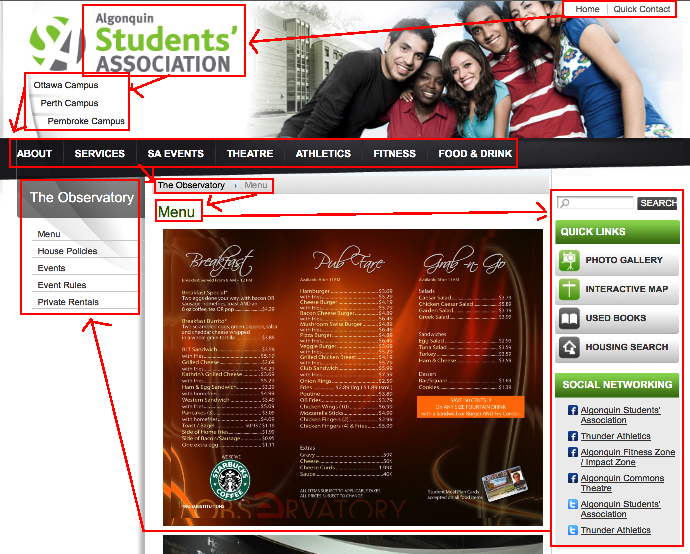
\includegraphics{alg_menu_vo_path.png}
\caption{Path VoiceOver follows through a document with an image with no
metadata. Note the arrows indicating the direction of travel; starting
from the top right at Home and Quick Contact, the path proceeds to the
SA logo, then the campus list, and then the navigation bar. The rest of
the path should be fairly evident. A transcript can be found in
\hyperref[transcript-of-an-inaccessible-page-with-an-image]{Appendix
A}\label{menuimg}}
\end{figure}

\clearpage

One of the other types of content that is impossible for software to
interpret, regardless of provisions made, is flash content. Flash
content is effectively a black box to screen readers as flash is a
binary, rather than text-based, format and is basically a computer
program in it's own right. It is possible for authors of flash content
to embed screen reading software into the flash application but that is
entirely up to the flash author and may be completely outside the
control of the web page author. All a web page author can do is annotate
the area the flash applet resides in with metadata, anything else must
be done in the flash applet itself. Without this metadata, the object is
invisible to the end user. The same software mentioned above, VoiceOver,
has exactly the same issue with flash as it does with metadata-less
images, as shown in Figure \ref{flashgal}.

\begin{figure}[htbp]
\centering
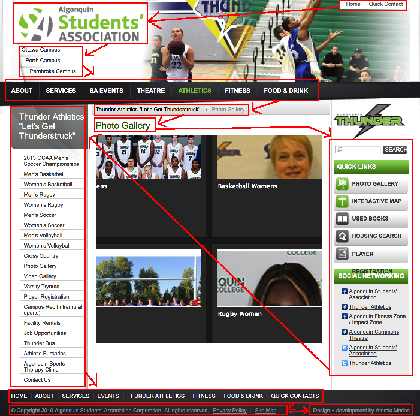
\includegraphics{alg_gal_vo_path.png}
\caption{Path VoiceOver follows through a document with a flash video.
The path is identical to that of the page with an image.
\label{flashgal}}
\end{figure}

The standards referenced earlier describe several ways the above issues
can be mitigated. Primarily, the use of metadata is the easiest and
fastest way for content creators to make their content available to
consumers. Such metadata includes attributes such as ``alt'' and
``title'' for images, links, and objects such as flash. When attributes
such as these are attached to the portion of the document that specifies
the offending objects, the screen reader is able to read the metadata
and present it to the end user. In Figure \ref{winplayer}, the page has
the requisite tags and as such, the screen reader is able to pass the
contained information on to the end user.

\begin{figure}[htbp]
\centering
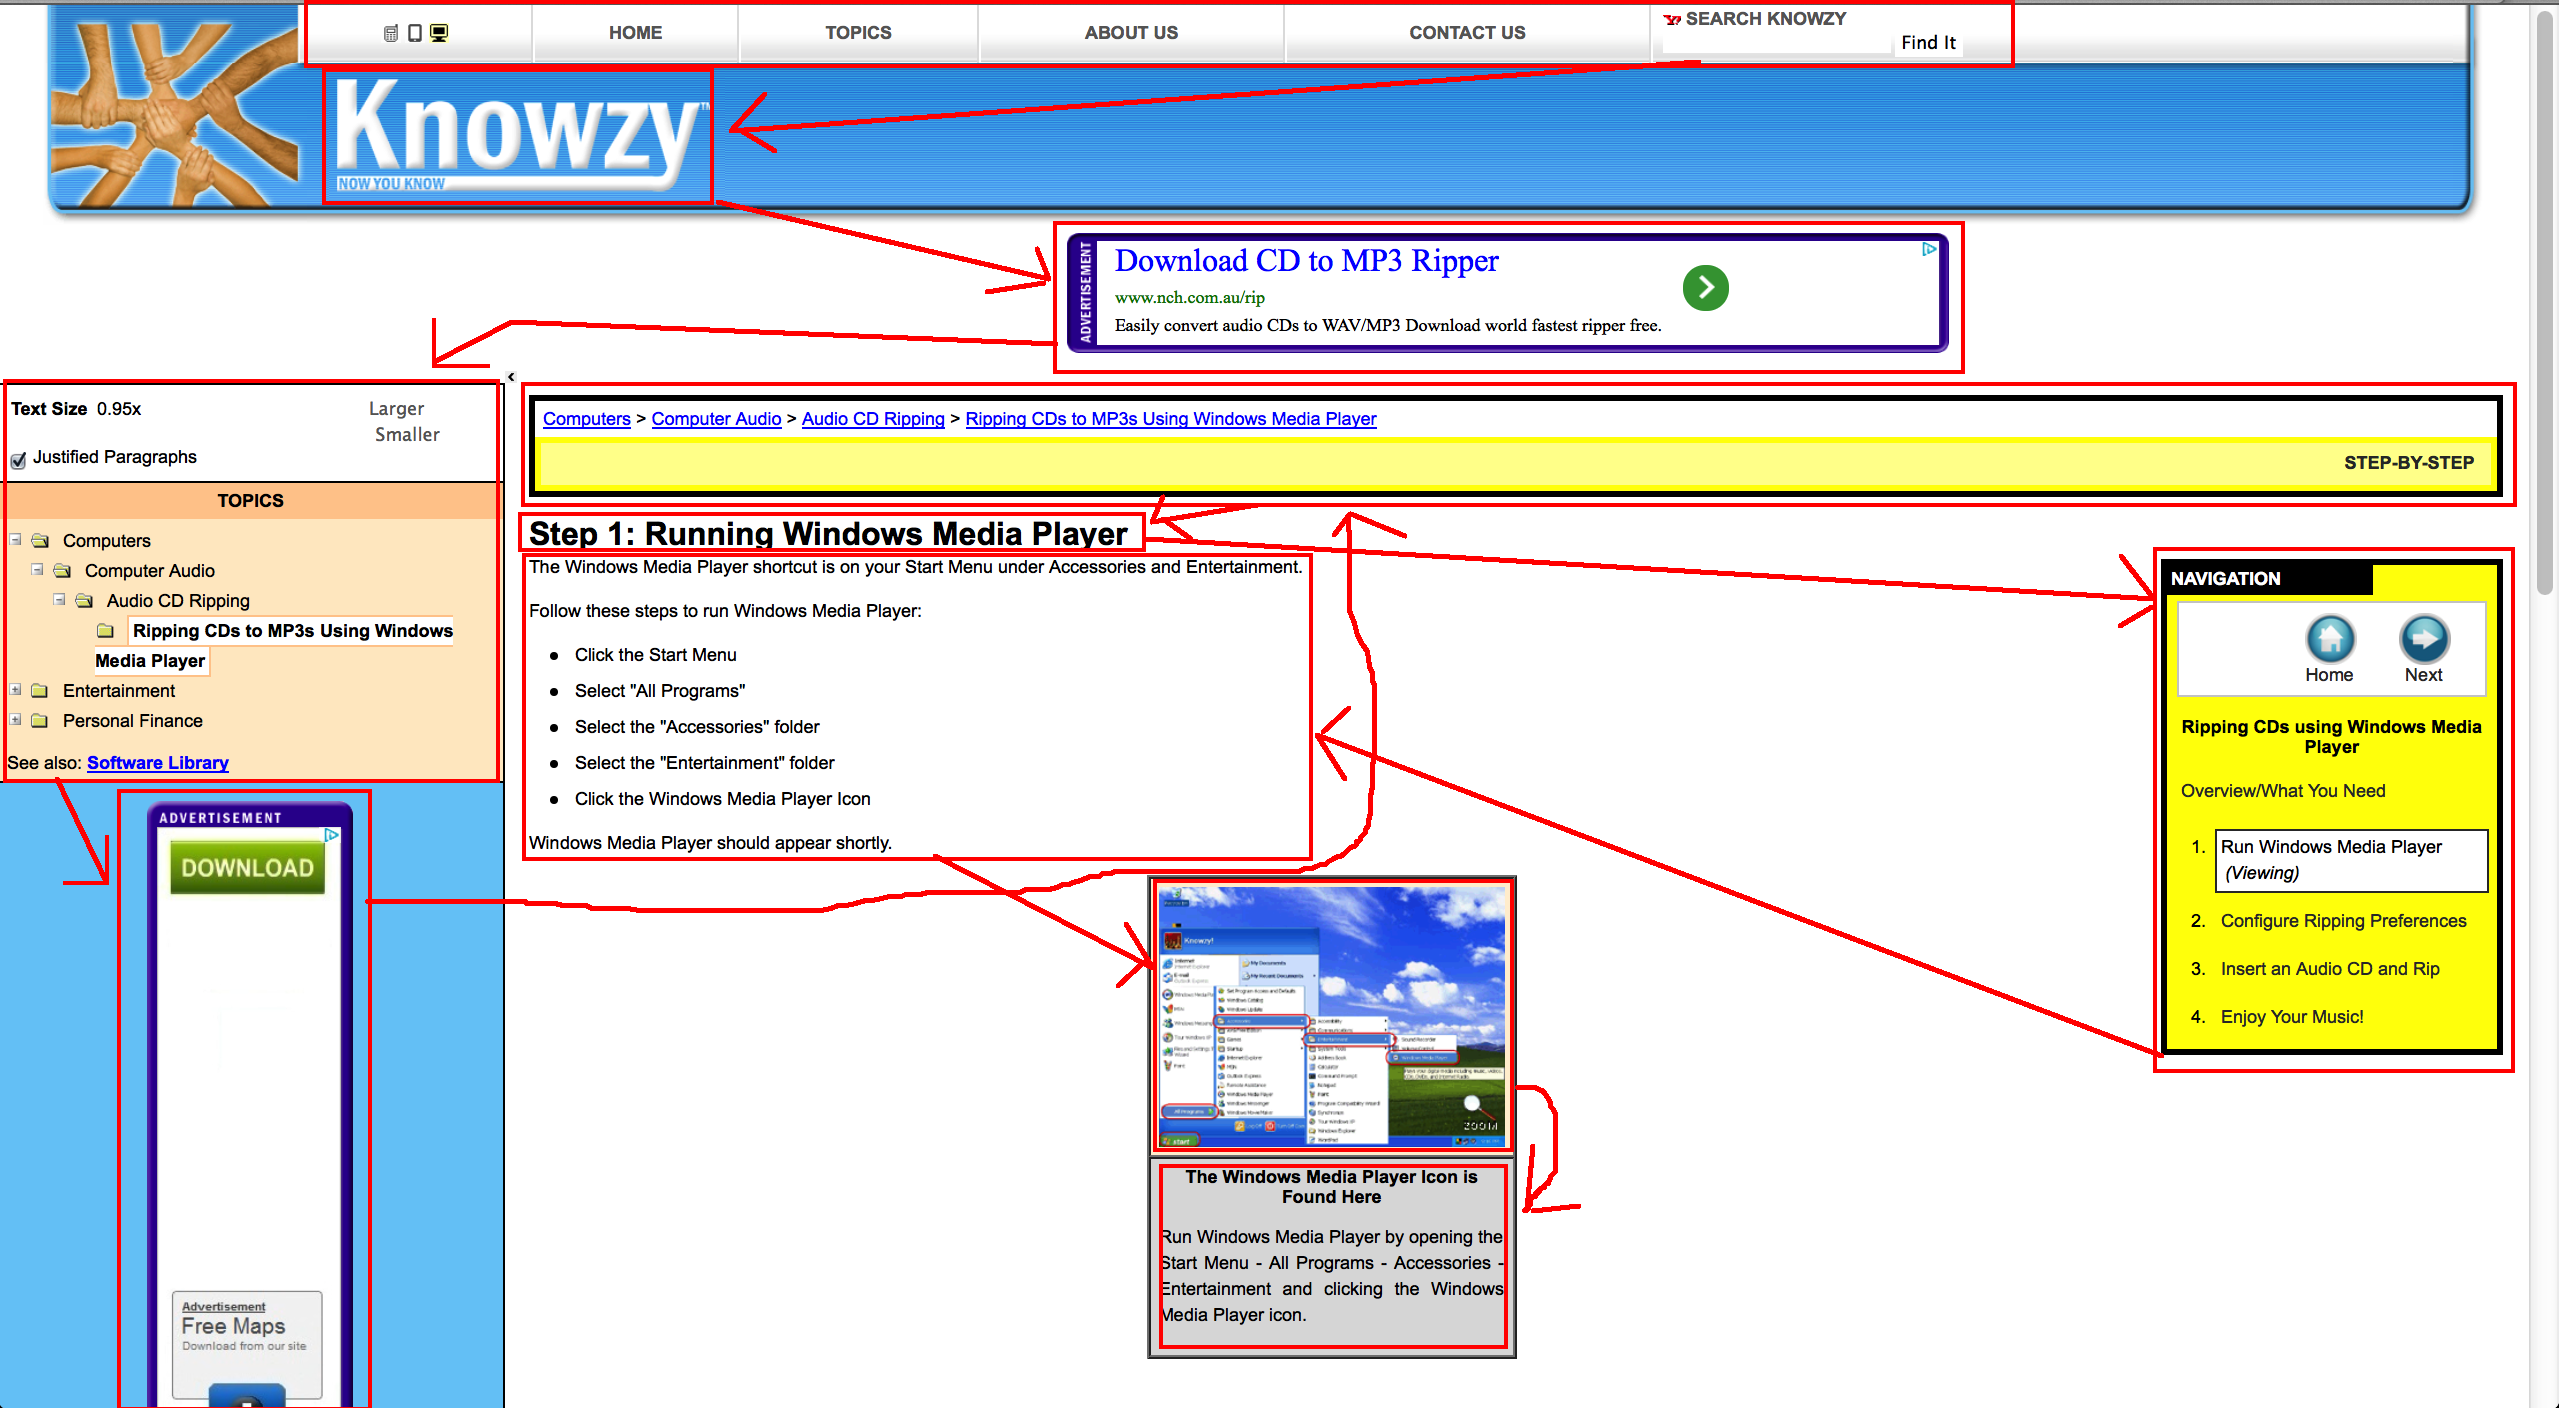
\includegraphics{win_player_vo_path.png}
\caption{Path VoiceOver follows through a document{[}8{]} with an image
with metadata. The path starts at the navigation bar at the top of the
page, proceeds to the logo, then the advertisement followed by the page
contents on the left. It proceeds upon a predictable path until the end
of the page however it may be difficult to see the path around the
image: it visits the image, describes it, and then reads the description
underneath it. The transcript can be found in
\hyperref[transcript-of-an-accessible-page-with-an-image]{Appendix A}
\label{winplayer}}
\end{figure}

\subsection{Current Situation At
Algonquin}\label{current-situation-at-algonquin}

The current situation at Algonquin is largely okay. Most of the site is,
in fact, accessible; the main content is presented fairly early on by
screen readers and the navigation is left to the end for most pages. In
the ideal page, this is desired as the user likely has knowledge of the
navigation elements already and is more interested in the main content.
Other areas of the site currently lack this layout, mainly due to the
main content being images or flash objects. Overall, the site is
accessible however has exceptions.

\subsubsection{Images}\label{images}

The first major accessibility failure is that existing photos such as
the menu for The Observatory{[}9{]} have no metadata associated with
them. The end user will quite literally skip over the image in the
document and have no idea there is even an image, they might even be
under the impression that the page is incomplete. This is a serious and
insurmountable obstacle for someone who wishes to peruse the menu as the
only other option is to visit the establishment and have someone read
off the menu. It may not even be possible for this to be an option as
other disabilities may be in play.

\subsubsection{Galleries}\label{galleries}

The other major accessibility failure is the use of flash-based
galleries. As mentioned before, this content is completely invisible to
the end user and therefore the aforementioned issues with images apply.

\subsection{Proposed Solution}\label{proposed-solution}

\subsubsection{Images}\label{images-1}

As referred to earlier, the use of alt and title attributes make the
page completely visible. Adding these attributes is simply a matter of
opening the relevant page in a text editor, finding the relevant image
in the document, and appending the requisite text.

Ideally, for information such as the menu for The Observatory, the
information would be extracted from the image and inserted into a table
while removing the original image.

Depending on the content management system used by the student
association, the difficulty of adding this data ranges from very easy,
in the case of using a point-and-click editor, to very difficult, in the
case of editing the page source code directly.

\subsubsection{Galleries}\label{galleries-1}

In current web development methodologies, the use of flash is deprecated
and a solution based on HTML, javascript, and CSS is preferred. Several
implementations exist on the internet and the addition of which is
usually a simple matter of removing the reference to the flash applet
and replacing it with HTML markup as required by the chosen
implementation. Usually, gallery implementations are written such that
if a user uses an alternative stylesheet or has javascript disabled, the
gallery degrades into a linear row or column of images. This is ideal in
that screen readers are unable to interpret CSS or javascript and as
such, merely see what would be on screen if either, or both, of the
aforementioned degradation conditions were true.

Alternatively, the author may migrate the images over to a site such as
Facebook, as has already been done with the SA event and The Observatory
photos. In this case, the work needed is minimal as Facebook has already
implemented the gallery and all the author needs to do is upload the
photos and provide captions.

\subsection{Cost}\label{cost}

The cost of making the Algonquin Student Association web site is fairly
minimal in both monetary and time costs. In terms of time, an afternoon
is all I expect a user would spend adding metadata to photos and
extracting textual content. The time to convert galleries from flash
would take a little longer as there is likely no ``drag-n-drop'' method
if the author chose to convert to a HTML+javascript+CSS-based solution.
If the author chose to use Facebook, the initial time investment would
be about the same but maintenance would be much cheaper.

In terms of monetary cost, the work involved is typically already a part
of the assigned author's duties so their would be no additional payment
upon completion. It's possible that the author may choose a gallery
implementation that requires payment however I personally know of no
such implementations. The optimal solution, Facebook, is free, so there
should be no cost to this project.

\subsection{Qualifications}\label{qualifications}

I've been developing software for almost 9 years. In that time, I've
developed countless tools for personal use to automate repetitive tasks
and ease my daily workload. Additionally, I've donated considerable time
over the past 3 years to the University of Ottawa's club, Humans vs
Infected, to develop and administer the web application used to manage
the game. The web application consists of content and player management
systems which use a range of technologies from HTML, javascript, and CSS
to Python and MySQL. Throughout the development of the website, I've
endeavoured to make the content accessible through the minimization of
image use, the complete lack of flash objects, and the overall layout of
the pages.

I'm also visually impaired myself. Although I don't require the use of a
screen reader, other parts of the standards deal with allowing the
content to re-arrange as the text size or window size change. I
frequently change the sizes of both to enable me to read content more
comfortably. During the course of my use of the internet, I've learned
how to adjust the source code of inaccessible pages to allow me to
change the sizes with the ultimate purpose of allowing the text to
re-arrange itself into shorter lines.

\clearpage

\section{Conclusion}\label{conclusion}

The standards dictate a lot of requirements for pages to be accessible,
however as they are standards, they need to account for every possible
situation. Based on the content currently on the Algonquin Student
Association website, the applicable changes are not onerous and won't
take a great deal of time to implement.

It's common belief that making a website accessible will impact
usability and design. Based on an interview with Léonie Watson{[}10{]},
this is not the case. There is absolutely no reason to not make websites
accessible. The SA website is fairly usable and has a pleasing design
and is still reasonably accessible in most cases so it is a case that
can be used to prove this point.

Based on an article{[}11{]} published by Laura O'Grady, more needs to be
done to make sites accessible. While the article was focussed on health
care sites, the fact is that the content is not specific to health care.
By making the SA website more accessible, we can help make the internet
more accessible for everyone.

For any questions, I can be contacted at
\href{mailto:r0ssar00@gmail.com}{r0ssar00@gmail.com}
or\\\href{mailto:r0ssar00@gmail.com}{ross0262@algonquinlive.com}.

\clearpage

\section*{References}\label{references}
\addcontentsline{toc}{section}{References}

{[}1{]}W3C, ``Web Content Accessibility Guidelines 2.0,''
\emph{Worldwide Web Consortium}, 11-Dec-2008.

{[}2{]}W3C, ``Techniques and Failures for Web Content Accessibility
Guidelines 2.0,'' \emph{Worldwide Web Consortium}, 05-Sep-2013.

{[}3{]}W3C, ``Accessible Rich Internet Applications (WAI\_ARIA) 1.0,''
\emph{Worldwide Web Consortium}, 2011.

{[}4{]}Treasury Board of Canada Secretariat, ``Standard on Web
Accessibility,'' \emph{Canada}, 2011.

{[}5{]}General Services Administration's Office of Governmentwide
Policy, ``Section 508,'' \emph{United States of America}.

{[}6{]}Ontario Government, ``Accessibility Standards for Customer
Service,'' 27-Jul-2007.

{[}7{]}Ontario Government, ``Accessibility for Ontarians with
Disabilities Act, 2005,'' 2005.

{[}8{]}Knowzy, ``Step 1: Run Windows Media Player,'' 14-Sep-2005.

{[}9{]}Algonquin Student Association, ``Menu,'' \emph{The Observatory}.

{[}10{]}Creative Blog, ``Léonie Watson: accessibility is not the enemy
of design,'' 2013.

{[}11{]}L. O'Grady, ``Accessibility compliance rates of
consumer-oriented Canadian health care Web sites,'' \emph{Medical
Informatics \& The Internet In Medicine}, vol. 30, no. 4, pp. 287--295,
Sep. 2005.

\clearpage

\section{Glossary}\label{glossary}

\begin{description}
\item[Source code]
Text that is translated into instructions by a computer.
\item[Compiled code (binary code)]
Data that only a machine can read. It is the list of instructions to be
executed.
\item[Rich Internet Applications (RIA)]
A RIA is a collection of javascript, html, and css that when combined by
a browser, produce an interactive website that behaves much like a
desktop application.
\item[HTML]
The markup language used to create the structure of web pages.
\item[Javascript]
The scripting language used to control web pages.
\item[CSS]
The language used to designate the style of web pages.
\item[Stylesheet]
A file containing CSS code
\item[Flash]
Browser plugin that allows for more complex applications than
HTML+Javascript+CSS typically allow.
\item[Flash applet]
A binary object that the browser downloads and executes in the flash
plugin.
\item[Depth-first traversal]
A method of performing an operation each element of a tree such that
each element is visited precisely once, the parent node is visited
before it's children, and the left side is visited before the right
side. For example:
\end{description}

\begin{verbatim}
    traverse GIVEN parent node:
        perform_operation ON parent node
        for every child of the parent node, from left to right:
            traverse SELECTED child node
\end{verbatim}

\clearpage

\subsection{Appendix A}\label{appendix-a}

\subsubsection{Transcript of an inaccessible page with an
image}\label{transcript-of-an-inaccessible-page-with-an-image}

\begin{verbatim}
list 2 items
link home
link quick contact
link image algonquin student association home
list 3 items
link ottawa campus
link perth campus
link pembroke campus
list 7 items
link about
link services
link sa events
link theatre
link athletics
link fitness
link food and drink
link the observatory menu
heading level 1 menu
site search edit text
search button
heading level 2 quick links
link photo gallery
link interactive map
link used books
link housing search
heading level 2 social networking
link algonquin student association
link thunder athletics
link algonquin fitness zone slash impact zone
link algonquin commons theatre
link algonquin students association
link thunder athletics
link the observatory
list 5 items
visited link menu
link house policies
link events
link event rules
link private rentals
list 8 items
visited link home
link about
link services
link events
link thunder athletics
link fitness
link food and drink
link quick contacts
copyright sign copyright 2010 algonquin students association corporation all rights reserved
list 2 items
link privacy policy
link site map
link design plus development by atomic motion
\end{verbatim}

\subsubsection{Transcript of an accessible page with an
image}\label{transcript-of-an-accessible-page-with-an-image}

\begin{verbatim}
internal link skip to main content
mobile view button button
smart view button button
desktop item image
link home
link topics browns topics at knowzy
link about us learn about knowzy
link contact us get in touch with knowzys
yahoo icon image
search k n o w z y
search k n o w z y search text field
find it button
link image knowzy know you know
frame 0
text size 095x
larger version
smaller version
justify paragraphs check checkbox
topics
list 3 items
link computers
list 1 item level 2
link computer audio
list 1 item level 3
link audio cd ripping
list 1 item level 4
link ripping cds to mp3s using windows media player
link entertainment
link personal finance
see also link software library
frame 3
link computers
link computer audio
link audio cd ripping
link ripping cds to mp 3 s using windows media player
step by step
heading level 1
step 1 running media player clickable
navigation
link image
step by step home icon
how to rip cds using windows media player overview
link image next page icon
step 2 configure ripping preferences
link home
how to rip cds using windows media player overview
link next step 2 configure ripping prefs
heading level 2 ripping cds using windows media player clickable
link overview slash what you need
list 4 items
1 run windows media player viewing group
1 run windows media player viewing
2 link configure ripping prefs
3 link insert an audio cd and rip
4 link enjoy your music
the windows media player shortcut is on your start menu under accessories and entertainment
follow these steps to run windows media player
list 5 items
bullet click the start menu
group
bullet click the start menu
bullet select all programs
group
bullet select all program
bullet select the accessories folder
group
bullet select the accessories folder
bullet select the entertainment folder
group
bullet select the entertainment folder
bullet click the windows media player icon
group
bullet click the windows media player icon
windows media player shouold appear shortly
row 1 of 2 column 1 of 1
link image screenshot of the start menu open with windows media player selected
click here to zoom if you are having trouble reading the text
row 2 of 2 column 1 of 1
the windows media player icon is found here
run windows media player by opening the start menu all programs accessories
entertainment and clicking the windows media player icon
note if you see an advertisement when the program starts
you probably need to upgrade to the link latest version of windows media player
microsoft's windows media player page
\end{verbatim}

\end{document}
